% Narrative source. build_report.py generates the pinned tables and figures only.
\documentclass[10pt,a4paper]{article}
\usepackage{fontspec}
\setmainfont{texgyretermes}[Extension=.otf,UprightFont=*-regular,BoldFont=*-bold,ItalicFont=*-italic,BoldItalicFont=*-bolditalic]
\usepackage[margin=1.8cm,headheight=14pt]{geometry}
\usepackage{amsmath,amssymb,booktabs,tabularx,array,ragged2e,enumitem,microtype,xcolor,tikz,fancyhdr,graphicx,titlesec}
\usetikzlibrary{arrows.meta,positioning}
\usepackage[hidelinks,unicode]{hyperref}
\definecolor{ink}{HTML}{183A45}
\definecolor{teal}{HTML}{087F7A}
\definecolor{blue}{HTML}{405F8A}
\definecolor{gray}{HTML}{56656B}
\definecolor{orange}{HTML}{976440}
\newcolumntype{P}[1]{>{\RaggedRight\arraybackslash}p{#1}}
\newcolumntype{Y}{>{\RaggedRight\arraybackslash}X}
\setlength{\parindent}{0pt}\setlength{\parskip}{5pt}\setlength{\emergencystretch}{2em}
\setlength{\tabcolsep}{4pt}\renewcommand{\arraystretch}{1.16}
\setlist{nosep,leftmargin=1.4em,topsep=3pt}
\titleformat{\section}{\large\bfseries\color{ink}}{\thesection}{.6em}{}
\titleformat{\subsection}{\normalsize\bfseries\color{ink}}{\thesubsection}{.6em}{}
\titlespacing*{\section}{0pt}{8pt}{6pt}
\titlespacing*{\subsection}{0pt}{7pt}{4pt}
\pagestyle{fancy}\fancyhf{}
\fancyhead[L]{\small\color{gray}BẢO VỆ RIÊNG TƯ BẰNG GEO-I / REM}
\fancyhead[R]{\small\color{gray}Cơ chế và bằng chứng}
\fancyfoot[C]{\small\thepage}\renewcommand{\headrulewidth}{0.3pt}
\newcommand{\key}[1]{\par\smallskip\noindent\textcolor{teal}{\textbf{#1}}\par\smallskip}
\hypersetup{pdftitle={Bảo vệ riêng tư truy vấn và quỹ đạo bằng Geo-I/REM},pdfauthor={}}
\newcommand{\UtilityRows}{Gần nhất & 92,45 & 94,68 & +2,23\\
Nhanh nhất & 92,45 & 94,68 & +2,23\\
Trong bán kính & 81,69 & 86,88 & +5,18\\
Ít vòng đường nhất & 92,27 & 94,52 & +2,25\\
Trung bình đều bốn mục đích & 89,71 & 92,69 & +2,97\\}
\newcommand{\CoordinateRows}{S1 & 100,00 & 5,56 & 1119 & 91,24\\
S2 & 100,00 & 1,39 & 874 & 97,98\\
S3 & 100,00 & 2,88 & 904 & 95,62\\}
\newcommand{\EndpointRows}{S9 & 1,79 & 790 & 0,00 & 1407\\
S10 & 0,00 & 758 & 0,00 & 1337\\}
\newcommand{\InferenceRows}{Chỉ khác một GPS, $r=10$ m & 0,20 & 54,98\%\\
Chỉ khác một GPS, $r=100$ m & 2,00 & 88,08\%\\
Cả trace, $D_\infty=100$ m, cap $0{,}23/\mathrm m$ & 23,00 & $\approx100\%$\\}
\newcommand{\TimelineRows}{0 & Có & Tạo mới & Cập nhật & 1u & 1/23\\
20 & Không & Giữ & Dự đoán & 0u & 1/23\\
60 & Có & Tạo mới & Cập nhật & 2u & 3/23\\
120 & Có & Tạo mới & Cập nhật & 2u & 5/23\\
600 & Có & Tạo mới & Cập nhật & 2u & 21/23\\}

\begin{document}
\begin{center}
{\LARGE\bfseries\color{ink}Bảo vệ riêng tư truy vấn và quỹ đạo}\\[3pt]
{\large Geo-I / REM, mạng đường và xử lý nhu cầu tại thiết bị}
\end{center}

\section{Nội dung truy vấn và ngân sách từng phiên}
\textbf{Nền tảng giữ nguyên:} GPS được bảo vệ bằng Geo-I/REM để tạo hoặc giữ tham chiếu $Z$.
Thiết bị ước lượng phân bố $b$ từ lịch sử đã bảo vệ, rồi chọn $K=5$ tọa độ truy vấn $Q$ khả thi theo mạng đường.
Máy chủ thấy $Q$ và lịch gửi, không nhận GPS thật, $Z$, nhu cầu $\psi$ hoặc đáp án local.

\subsection{S7: giữ nhu cầu thật local, truy hồi một tập ứng viên chung}
Nhu cầu thật $\psi$ gồm loại POI, tiêu chí, bán kính hoặc đích riêng. Máy chủ luôn nhận cùng yêu cầu:
mọi loại POI công khai, độ sâu cố định $L=30$ tại mỗi $Q$. Sau khi nhận phản hồi, thiết bị mới gộp,
bỏ trùng ID và dùng GPS cùng $\psi$ để lọc, sắp xếp danh sách phù hợp.
\[
5Q\times L30\ \longrightarrow\ \leq150\text{ bản ghi mỗi loại}
\ \longrightarrow\ \text{nhận, bỏ trùng}\ \longrightarrow\ \text{lọc và sắp xếp local}.
\]
Con số 150 là trần trước bỏ trùng, không phải 150 POI duy nhất hay trần cho toàn bộ sáu loại POI.
Truy hồi mọi loại đã có từ trước; phần mở rộng là bốn nhu cầu local và kiểm tra yêu cầu mạng bất biến khi đổi nhu cầu.

\par\smallskip
\begin{tabularx}{\linewidth}{@{}P{3.4cm}Y@{}}\toprule
\textbf{Nhu cầu local} & \textbf{Tiêu chí lọc / sắp xếp}\\\midrule
Gần nhất & Khoảng cách đường $D_G(x,p)$.\\
Đến nhanh nhất & Thời gian đường thông thoáng $T_G(x,p)$; chưa gồm ùn tắc.\\
Trong bán kính $r$ & Giữ $D_G(x,p)\leq r$, rồi sắp theo khoảng cách.\\
Ít đi vòng tới đích $a$ & $D_G(x,p)+D_G(p,a)-D_G(x,a)$; đích $a$ chỉ dùng local.\\\bottomrule
\end{tabularx}

\key{S7: cùng trạng thái đã bảo vệ và lịch công khai, đổi nhu cầu $\psi$ không đổi $Q$, payload, lịch hoặc số request.}
Độ gần là cách thu ứng viên cho dịch vụ lân cận, không bắt mọi nhu cầu chọn POI gần nhất.
Đủ đáp án chỉ khi pool chứa các POI cần thiết. Số POI hiển thị không quyết định cơ chế S7;
triển khai và benchmark vẫn dùng $k=5$, Recall@5. Tương quan ý định--tuyến đường và click còn là kênh suy luận.

\subsection{Ngân sách Geo-I theo từng phiên}
Một phiên là một chuyến/lượt sử dụng, gồm nhiều lần đọc GPS và gửi Q. Khởi động lại để tiếp tục cùng chuyến không tự nạp ngân sách.
Với cap hiệu lực $C_s$, tham số phân bổ $H$ công khai và $U=2H-1$:
\[
u=C_s/U,\qquad B_{\rm nominal}=2Hu.
\]
Cấu hình làm việc: $C_s=0{,}23\,\mathrm m^{-1}$, $H=12$, $U=23$, $u=0{,}01\,\mathrm m^{-1}$, $B=0{,}24\,\mathrm m^{-1}$.
Đây là hệ số riêng tư, không phải bán kính nhiễu; công thức phân bổ không chứng minh $0{,}23$ tối ưu cho mọi dữ liệu.
\par\smallskip
\begin{tabularx}{\linewidth}{@{}Ycccc@{}}\toprule
\textbf{Nhánh} & Đọc đầu & Thử, giữ $Z$ & Thử, tạo $Z$ & Không đọc\\\midrule
\textbf{Chi phí} & $1u$ & $1u$ & $2u$ & $0u$\\\bottomrule
\end{tabularx}
Dự toán trước GPS: lần đầu đủ $1u$, các lần sau đủ $2u$; hai lần đọc cách ít nhất 60 s.
Không đọc mới thì dự đoán từ lịch sử bảo vệ. $H$ không phải số lần đọc GPS tối đa.
Trong mô hình lý tưởng, toàn transcript $E$ của một phiên có chặn:
\[
\Pr[E\in A\mid X]\leq e^{C_sD_\infty(X,X')}\Pr[E\in A\mid X'].
\]
$D_\infty$ là khoảng cách lớn nhất giữa các vị trí tương ứng của hai trace.
Nhiều phiên liên kết vẫn hợp thành tổng cap. Cận giả định miền đường/lịch công khai, thiết bị tin cậy,
REM và phép thử lý tưởng; chưa chứng nhận sampler số thực.
\clearpage
\section{S4--S6: phân tích mức bảo vệ từ cận Geo-I}
\begingroup\setlength{\parskip}{3pt}\renewcommand{\arraystretch}{1.06}
S4--S6 xét danh tính hoặc lựa chọn tương lai: trọng tâm là cận thay đổi niềm tin của attacker.
Diagnostic đã lưu giữ để tra cứu; benchmark tọa độ S1--S3, S9--S10 ở mục 6.

\subsection{Từ tọa độ đến giả thuyết về secret}
Gọi $\mathsf O$ là toàn transcript máy chủ thấy: các Q và lịch công khai; $P_0,P_1$ là hai luật của $\mathsf O$
dưới giả thuyết $H_0,H_1$. REM, phép thử tái sử dụng và cap cho chặn lý tưởng của tọa độ;
$b$, chọn Q và truy hồi chung là hậu xử lý từ lịch sử đã bảo vệ, không thêm GPS thô.
Để chuyển chặn này sang secret, cần cùng ngữ cảnh công khai và \emph{mọi cặp trace giữa hai support}
thỏa $D_{\infty,s}\leq r_s$. Khi đó:
\[
 \alpha=\sum_s C_s r_s,\qquad
 P_0(A)\leq e^\alpha P_1(A),\quad P_1(A)\leq e^\alpha P_0(A).
\]
Lấy tích phân qua hai phân phối trace cho chặn giả thuyết. Gần nhau tại một GPS chưa đủ chặn hai nhóm hành trình.

\subsection{Attacker học thêm được bao nhiêu?}
Với prior $\pi\in(0,1)$ của $H_1$, tại event quan sát $A$ có xác suất dương:
\[
 e^{-\alpha}\leq
 \frac{\Pr[H_1\mid A]/\Pr[H_0\mid A]}{\pi/(1-\pi)}
 \leq e^\alpha.
\]
Nghĩa là quan sát chỉ nhân tỷ lệ tin giữa hai giả thuyết tối đa $e^\alpha$.
Cận xét \textbf{thông tin tăng thêm}, không xóa tri thức trước của attacker.
Với prior cân bằng, $\operatorname{TV}(P_0,P_1)\leq\tanh(\alpha/2)$ cho:
\[
 \Pr[\text{Bayes đoán đúng}]\leq\frac{e^\alpha}{1+e^\alpha}.
\]
Với $M$ giả thuyết có prior đều và \emph{mọi cặp} thỏa cùng chặn,
$\Pr[H=j\mid A]\leq e^\alpha/(e^\alpha+M-1)$.
$M$ là số giả thuyết về secret, không phải $K=5$ tọa độ Q.

\subsection{Áp dụng riêng cho S4, S5 và S6}
\par\smallskip
\begin{tabularx}{\linewidth}{@{}P{.75cm}P{3.25cm}Y@{}}\toprule
\textbf{Case} & \textbf{Secret và giả thuyết} & \textbf{Ý nghĩa và điều kiện của cận}\\\midrule
S4 & Cùng người / cùng xe vật lý & So cặp transcript dưới cùng/khác chủ thể; tính cap mọi phiên quan sát và chặn mọi cặp trace giữa hai nhóm. Người đổi xe khác với hai người chung xe; số Q không tự cho chặn identity.\\
S5 & Cạnh đường sẽ đi tiếp & So prefix giữa các cạnh ứng viên. Prefix thật/ngữ cảnh giống thì luật Q giống: không thêm thông tin về lựa chọn tương lai. Khi có dấu hiệu rẽ, dùng chặn khoảng cách prefix; không dùng GPS tương lai.\\
S6 & Điểm đến chưa tới & So lịch sử + prefix giữa các đích; cộng cap các phiên đã liên kết. Prior routine có thể mạnh. Đích private local không lộ trực tiếp qua payload; hành trình vẫn có thể gợi ý đích.\\\bottomrule
\end{tabularx}
S4 áp dụng riêng người/xe, không thay bằng ID thiết bị. S6 giả định lịch sử đã liên kết không chứng minh S4.
Chưa chọn thêm k-anonymity trước khi xác định thiếu bảo vệ của mô hình.

\subsection{Ví dụ định lượng và giới hạn của kết luận}
Với $u=0{,}01/\mathrm m$, hai trace chỉ khác \textbf{một mẫu GPS} cách $r$ có $\alpha\leq2ur$
cho toàn transcript, kể cả ảnh hưởng đến các Q sau đó. Hai trace khác nhiều mẫu dùng cận cap phiên.
\par\smallskip
\begin{tabularx}{\linewidth}{@{}Yrr@{}}\toprule
\textbf{So sánh giả thuyết, prior cân bằng} & \textbf{$\alpha$} & \textbf{Cận Bayes}\\\midrule
\InferenceRows
\bottomrule\end{tabularx}
Đây là cận lý thuyết, \textbf{không phải accuracy benchmark}. Một mẫu không đại diện hai tuyến bất kỳ;
cận gần 100\% chưa hữu ích để chứng minh bảo vệ mạnh.
Kernel lý tưởng, thiết bị tin cậy và lịch/ngữ cảnh chung là điều kiện; account/IP và sampler float chưa được chứng nhận.

\key{S4--S6: đã có công thức để phân tích mức bảo vệ có điều kiện; chưa suy thành ẩn danh hoặc chống mọi dự đoán tương lai.}
Metrics theo secret: S4 linkage dùng AUC/BA; S5 dùng đúng cạnh; S6 dùng đúng đích/Hit100 và MAE.
Có thể chia sẻ metric phù hợp, không dùng một score cho tất cả. S8 còn mở.
{\footnotesize\color{gray}Nguồn: \href{https://arxiv.org/html/1212.1984v3}{Geo-I (Andrés et al., 2013)},
\href{https://arxiv.org/html/1311.4008v2}{predictive composition (Chatzikokolakis et al., 2014)};
\texttt{current\_formal\_privacy.tex}, \texttt{current\_formal\_inference.tex}. Đây là hệ quả của Geo-I, không phải primitive riêng tư mới.}

\endgroup
\clearpage
\section{Kiến trúc trước: cap từng phiên và tìm POI gần nhất}
Đọc từ trên xuống theo các bước đánh số. Khung xanh là mô hình tại thiết bị; máy chủ POI ở ngoài khung.
Mũi tên liền thể hiện luồng chính, nét đứt thể hiện dữ liệu công khai hoặc chính sách tùy chọn.
\begin{center}\begin{tikzpicture}[x=1cm,y=1cm,>=Latex,
      stage/.style={draw=ink!55,fill=white,rounded corners=2pt,text width=8.45cm,
                    align=center,inner sep=7pt,font=\small,minimum height=1.28cm},
      input/.style={draw=blue!65,fill=blue!3,rounded corners=2pt,align=center,
                    inner sep=6pt,font=\small},
      external/.style={draw=blue!65,fill=blue!3,rounded corners=2pt,text width=2.55cm,
                    align=center,inner sep=6pt,font=\small},
      flow/.style={->,line width=.85pt,draw=ink},
      network/.style={->,line width=.85pt,draw=blue},
      public/.style={->,dashed,line width=.65pt,draw=gray},
      layer/.style={text width=2.35cm,align=left,font=\small\bfseries,text=teal}]
    \fill[teal!2,rounded corners=4pt] (.5,-1.1) rectangle (12.9,-16.25);
    \draw[teal,line width=1pt,rounded corners=4pt] (.5,-1.1) rectangle (12.9,-16.25);
    \node[anchor=west,font=\small\bfseries,text=teal] at (.85,-1.45) {MÔ HÌNH TẠI THIẾT BỊ};
    \node[input,text width=3.3cm] (pub) at (1.95,.2) {\textbf{Dữ liệu công khai}\\Bản đồ, POI, lịch gửi};
    \node[input,text width=7.6cm] (gps) at (8,.2) {\textbf{GPS cho cơ chế Geo-I}\\Chỉ đọc sau khi lịch và ngân sách cho phép};
    \node[layer] at (1.95,-2.7) {Tầng 1\\Bảo vệ GPS};
    \node[stage,draw=ink,line width=.9pt] (guard) at (8,-2.8) {\textbf{1. Kiểm tra lịch và ngân sách}\\Cap $0{,}23/\mathrm m$ mỗi phiên; khoảng đọc $\geq60$ s\\Warmup 60 s trước GPS khi bật bảo vệ đầu chuyến};
    \node[stage] (rem) at (8,-5.05) {\textbf{2. Geo-I / REM + kiểm tra tái sử dụng}\\Đọc GPS $x$; thử giữ $Z$ bằng phép thử có nhiễu.\\Giữ $Z$ hoặc lấy mẫu REM mới trên miền đường cố định.};
    \draw[flow] (gps.south) -- (guard.north);
    \draw[flow] (guard.south) -- node[right,font=\footnotesize] {được phép đọc} (rem.north);
    \node[layer] at (1.95,-7.2) {Tầng 2\\Ước lượng và\\chọn truy vấn};
    \node[stage] (belief) at (8,-7.4) {\textbf{3. Ước lượng phân bố $b$ trên mạng đường}\\Đọc được: cập nhật từ quan sát đã bảo vệ.\\Không đọc mới: dự đoán từ lịch sử và chuyển tiếp công khai.};
    \node[stage] (planner) at (8,-9.45) {\textbf{4. Chọn 5 tọa độ truy vấn $Q$}\\Phủ POI; giới hạn chuyển động theo mạng đường.\\Bảng planner $L_{\rm plan}=10$; slack $0{,}03$ trên điểm độ phủ.};
    \draw[flow] (rem.south) -- node[right,font=\footnotesize] {$Z$ nội bộ} (belief.north);
    \draw[flow] (belief.south) -- (planner.north);
    \draw[flow] (guard.east) -- (12.65,-2.8) -- (12.65,-7.4) -- (belief.east);
    \node[rotate=90,font=\footnotesize,text=gray,fill=white,inner sep=2pt] at (12.65,-5) {không đọc GPS mới};
    \draw[public] (pub.south) -- (1.95,-.7) -- (.15,-.7) -- (.15,-9.45) -- (planner.west);
    \draw[public] (.15,-7.4) -- (belief.west);
    \node[layer] at (1.95,-11.65) {Tầng 3\\Truy hồi POI};
    \node[stage,draw=ink,line width=.9pt] (send) at (8,-11.7) {\textbf{5. Yêu cầu chung; delay tùy chọn}\\$K=5$ Q; mọi loại POI; $L=10$ mỗi loại mỗi Q\\Khi bật: giữ Q 60 s rồi mới công bố};
    \draw[flow] (planner.south) -- (send.north);
    \node[external,minimum height=1.9cm] (server) at (14.85,-11.7) {\textbf{MÁY CHỦ POI}\\Ngoài mô hình\\Trả top-$L$ mỗi loại\\tại từng $Q$};
    \draw[network] (send.east) -- node[above,font=\footnotesize] {$Q$} (server.west);
    \node[font=\small,text=gray,align=center,text width=8cm] at (8,-13.5) {$Z$ và GPS thật giữ tại thiết bị.\\Máy chủ chỉ nhận tọa độ $Q$ và yêu cầu chung.};
    \node[layer] at (1.95,-15.05) {Tầng 4\\Xử lý local};
    \node[stage,draw=ink,line width=.9pt] (local) at (8,-15.05) {\textbf{6. Hợp phản hồi và xếp hạng local}\\Giữ phản hồi còn hiệu lực theo epoch dịch vụ\\Xếp hạng gần nhất theo GPS; giới hạn $k=5$};
    \draw[network] (server.east) -- (16.75,-11.7) -- (16.75,-15.05) -- node[above,font=\footnotesize] {phản hồi POI} (local.east);
    \node[external,draw=orange,fill=orange!4,font=\footnotesize] (close) at (14.85,-13.75) {\textbf{Khi đóng phiên}\\Hủy Q còn chờ\\nếu đang bật delay};
    \draw[->,dashed,draw=orange] (send.south east) -- (12.95,-12.55) -- (12.95,-13.75) -- (close.west);
    \node[input,text width=4.6cm] (private) at (3.3,-17.3) {\textbf{Đầu vào riêng cho local}\\GPS local};
    \node[input,text width=4.6cm,draw=teal,fill=teal!4] (answer) at (10.15,-17.3) {\textbf{Đầu ra riêng cho người dùng}\\Tối đa 5 POI mỗi loại\\theo khoảng cách gần nhất};
    \draw[network] (private.north) -- (3.3,-16.45) -- (6,-16.45) -- (6,-15.82);
    \draw[flow,draw=teal] (10.15,-15.82) -- (answer.north);
    \end{tikzpicture}
\end{center}
\textbf{Bản trước:} $u=0{,}01/\mathrm m$, cap phiên $0{,}23/\mathrm m$, $K=5$, phản hồi $L10$;
xếp hạng gần nhất và chọn tối đa năm POI mỗi loại. Không đọc mới thì đi thẳng tới ước lượng $b$.

\textbf{S9/S10 tùy chọn:} warmup 60 s trước GPS, delay công bố 60 s, hủy Q còn chờ khi đóng.
Ví dụ đã lưu: Q tạo ở 60 s gửi ở 120 s; đóng tại 384 s hủy Q(340), Q(360), Q(380), Q(384).
Delay làm chậm hoặc mất câu trả lời; sơ đồ này mô tả nhánh lịch sử, không phải cấu hình L30 đã đo.

\clearpage
\section{Kiến trúc hiện tại: Geo-I và xử lý nhu cầu local}
Giữ Geo-I/REM, tái sử dụng $Z$, ước lượng $b$ và bộ chọn $Q$ theo đường.
Khung xanh là mô hình tại thiết bị; máy chủ ở ngoài. Các bước 1--6 thể hiện thứ tự xử lý;
viền xanh ở bước 5--6 đánh dấu phần mở rộng truy hồi và xử lý nhu cầu.
\begin{center}\begin{tikzpicture}[x=1cm,y=1cm,>=Latex,
      stage/.style={draw=ink!55,fill=white,rounded corners=2pt,text width=8.45cm,
                    align=center,inner sep=7pt,font=\small,minimum height=1.28cm},
      input/.style={draw=blue!65,fill=blue!3,rounded corners=2pt,align=center,
                    inner sep=6pt,font=\small},
      external/.style={draw=blue!65,fill=blue!3,rounded corners=2pt,text width=2.55cm,
                    align=center,inner sep=6pt,font=\small},
      flow/.style={->,line width=.85pt,draw=ink},
      network/.style={->,line width=.85pt,draw=blue},
      public/.style={->,dashed,line width=.65pt,draw=gray},
      layer/.style={text width=2.35cm,align=left,font=\small\bfseries,text=teal}]
    \fill[teal!2,rounded corners=4pt] (.5,-1.1) rectangle (12.9,-16.25);
    \draw[teal,line width=1pt,rounded corners=4pt] (.5,-1.1) rectangle (12.9,-16.25);
    \node[anchor=west,font=\small\bfseries,text=teal] at (.85,-1.45) {MÔ HÌNH TẠI THIẾT BỊ};
    \node[input,text width=3.3cm] (pub) at (1.95,.2) {\textbf{Dữ liệu công khai}\\Bản đồ, POI, lịch gửi};
    \node[input,text width=7.6cm] (gps) at (8,.2) {\textbf{GPS cho cơ chế Geo-I}\\Chỉ đọc sau khi lịch và ngân sách cho phép};
    \node[layer] at (1.95,-2.7) {Tầng 1\\Bảo vệ GPS};
    \node[stage,draw=ink,line width=.9pt] (guard) at (8,-2.8) {\textbf{1. Kiểm tra lịch và ngân sách}\\Cap $C_s=0{,}23\,\mathrm m^{-1}$ mỗi phiên\\Dự toán trước GPS; $u=0{,}01\,\mathrm m^{-1}$; khoảng đọc $\geq60$ s};
    \node[stage] (rem) at (8,-5.05) {\textbf{2. Geo-I / REM + kiểm tra tái sử dụng}\\Đọc GPS $x$; thử giữ $Z$ bằng phép thử có nhiễu.\\Giữ $Z$ hoặc lấy mẫu REM mới trên miền đường cố định.};
    \draw[flow] (gps.south) -- (guard.north);
    \draw[flow] (guard.south) -- node[right,font=\footnotesize] {được phép đọc} (rem.north);
    \node[layer] at (1.95,-7.2) {Tầng 2\\Ước lượng và\\chọn truy vấn};
    \node[stage] (belief) at (8,-7.4) {\textbf{3. Ước lượng phân bố $b$ trên mạng đường}\\Đọc được: cập nhật từ quan sát đã bảo vệ.\\Không đọc mới: dự đoán từ lịch sử và chuyển tiếp công khai.};
    \node[stage] (planner) at (8,-9.45) {\textbf{4. Chọn 5 tọa độ truy vấn $Q$}\\Phủ POI; giới hạn chuyển động theo mạng đường.\\Bảng planner $L_{\rm plan}=10$; slack $0{,}03$ trên điểm độ phủ.};
    \draw[flow] (rem.south) -- node[right,font=\footnotesize] {$Z$ nội bộ} (belief.north);
    \draw[flow] (belief.south) -- (planner.north);
    \draw[flow] (guard.east) -- (12.65,-2.8) -- (12.65,-7.4) -- (belief.east);
    \node[rotate=90,font=\footnotesize,text=gray,fill=white,inner sep=2pt] at (12.65,-5) {không đọc GPS mới};
    \draw[public] (pub.south) -- (1.95,-.7) -- (.15,-.7) -- (.15,-9.45) -- (planner.west);
    \draw[public] (.15,-7.4) -- (belief.west);
    \node[layer] at (1.95,-11.65) {Tầng 3\\Truy hồi POI};
    \node[stage,draw=teal,line width=.9pt] (send) at (8,-11.7) {\textbf{5. Yêu cầu chung, gửi ngay}\\$K=5$ Q; mọi loại POI; $L=30$ mỗi loại mỗi Q};
    \draw[flow] (planner.south) -- (send.north);
    \node[external,minimum height=1.9cm] (server) at (14.85,-11.7) {\textbf{MÁY CHỦ POI}\\Ngoài mô hình\\Trả top-$L$ mỗi loại\\tại từng $Q$};
    \draw[network] (send.east) -- node[above,font=\footnotesize] {$Q$} (server.west);
    \node[font=\small,text=gray,align=center,text width=8cm] at (8,-13.5) {$Z$ và GPS thật giữ tại thiết bị.\\Máy chủ chỉ nhận tọa độ $Q$ và yêu cầu chung.};
    \node[layer] at (1.95,-15.05) {Tầng 4\\Xử lý local};
    \node[stage,draw=teal,line width=.9pt] (local) at (8,-15.05) {\textbf{6. Gộp, bỏ trùng, lọc và sắp xếp local}\\GPS + nhu cầu $\psi$: gần nhất, nhanh nhất,\\trong bán kính hoặc ít đi vòng tới đích};
    \draw[network] (server.east) -- (16.75,-11.7) -- (16.75,-15.05) -- node[above,font=\footnotesize] {phản hồi POI} (local.east);

    \node[input,text width=4.6cm] (private) at (3.3,-17.3) {\textbf{Đầu vào riêng cho local}\\GPS local + nhu cầu $\psi$};
    \node[input,text width=4.6cm,draw=teal,fill=teal!4] (answer) at (10.15,-17.3) {\textbf{Đầu ra riêng cho người dùng}\\Danh sách POI phù hợp\\đã lọc và sắp xếp};
    \draw[network] (private.north) -- (3.3,-16.45) -- (6,-16.45) -- (6,-15.82);
    \draw[flow,draw=teal] (10.15,-15.82) -- (answer.north);
    \end{tikzpicture}
\end{center}
\textbf{So với bản trước:} $L10\to L30$ để tăng pool ứng viên; từ xếp hạng gần nhất mở rộng
thành bốn nhu cầu local. $K=5$, $L_{\rm plan}=10$, slack $0{,}03$ và nền Geo-I giữ nguyên.
Chính sách làm việc: cap phiên $0{,}23/\mathrm m$, $u=0{,}01/\mathrm m$; chưa có benchmark mới cho kết hợp cap này với L30.

\textbf{Liên hệ scenario:} tầng 1 làm mờ GPS cho S1--S3 và giảm tín hiệu linkage/dự báo S4--S6;
tầng 2 duy trì utility khi không đọc mới, không phải một bảo đảm identity độc lập;
tầng 3--4 giữ nhu cầu riêng local cho S7. Cận bảo vệ có điều kiện cho S4--S6 được phân tích riêng ở mục 2.

\textbf{Đầu/cuối:} nhánh delay là tùy chọn lịch sử. Nhánh Endpoint20 riêng tăng nhiễu ở mọi lần đọc và gửi ngay;
chưa gán kết quả nhánh đó cho kiến trúc L30. Chưa thêm khối k-anonymity hay lớp identity mới vào mô hình.
\clearpage
\section{Ví dụ cơ chế đã lưu: từ GPS đến danh sách POI}
Mẫu cố định \texttt{freshqp-001}, TRAIN, draw 1, phiên 1, \textbf{cấu hình minh họa đã lưu}, $u=0{,}00125/\mathrm m$, cap phiên $0{,}02875/\mathrm m$. Tham số khác cấu hình làm việc; không phải mẫu mới.
Mỗi mốc công khai 20 s gửi $Q$; lịch GPS cho Geo-I ít nhất 60 s. $Z$ giữ nội bộ, $Q$ gửi máy chủ, $P$ là POI trong danh mục.

\begin{minipage}[t]{.49\linewidth}\vspace{0pt}
\textbf{Thành phần kích hoạt theo thời gian}\par\smallskip
\begingroup\small\setlength{\tabcolsep}{3pt}
\begin{tabular}{@{}rlllll@{}}\toprule
$t$ (s) & GPS & $Z$ & $b$ & Phí & Tổng\\\midrule
\TimelineRows
\bottomrule\end{tabular}\endgroup

Ở 20 s, không đọc GPS mới: giữ $Z$, $b$ chỉ dự đoán, không chi thêm.
$Q$ vẫn có thể thay đổi theo lịch sử và mạng đường.
\end{minipage}\hfill
\begin{minipage}[t]{.49\linewidth}\vspace{0pt}
\textbf{Tại 60 s: GPS, $Z$, $b$ và năm $Q$}\\[3pt]
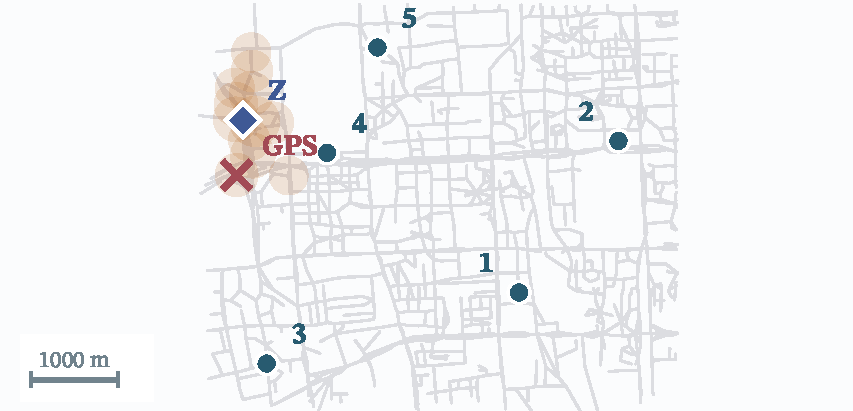
\includegraphics[width=\linewidth]{report_figures/sample_60s.pdf}
{\footnotesize Dấu chéo: GPS; hình thoi: $Z$; điểm 1--5: $Q$.
Màu cam: một phần trọng số $b$, không phải posterior hiệu chuẩn.
© OpenStreetMap contributors.}
\end{minipage}

\subsection{Tại 60 s: lần lượt kích hoạt các cơ chế}
\begin{enumerate}
\item \textbf{Lịch và ngân sách:} đủ 60 s từ lần đọc trước, còn 22/23 đơn vị; dành đủ dự toán $2u$ rồi mới đọc GPS.
\item \textbf{Thử giữ tham chiếu:} khoảng cách GPS tới $Z$ cũ là $3.049{,}59$ m,
$\theta=200$ m, nhiễu $\mathrm{Lap}(800\text{ m})$. Log lưu nhánh thử không đạt, không lưu giá trị nhiễu cụ thể.
\item \textbf{Geo-I/REM:} tạo $Z$ mới. GPS $(39{,}982839;116{,}292335)$;
$Z=(39{,}988552;116{,}293209)$. Chi thêm $2u=0{,}0025/\mathrm m$;
tổng $3u=0{,}00375/\mathrm m$, còn $0{,}025/\mathrm m$.
\item \textbf{Ước lượng và chọn Q:} cập nhật $b$ từ quan sát bảo vệ; chọn năm Q để phủ POI và tiếp tục di chuyển theo đường.
Không dùng GPS thật hoặc nhu cầu riêng để sửa Q.
\item \textbf{Truy hồi chung:} năm Q, L30 mọi loại, gửi ngay. Tổng phản hồi 420 bản ghi;
thiết bị gộp và bỏ trùng còn 252 POI duy nhất qua các loại.
\item \textbf{Nhu cầu local:} dùng GPS và $\psi$ để lọc, sắp xếp trên cùng phản hồi.
Không gửi thêm query khi đổi loại POI, tiêu chí, bán kính hoặc đích riêng.
\end{enumerate}

\par\smallskip
\begin{tabularx}{\linewidth}{@{}P{3.8cm}Y@{}}\toprule
\textbf{Nhu cầu: quán cà phê} & \textbf{Trích kết quả đã lưu, cùng phản hồi tại 60 s}\\\midrule
Gần nhất & Đầu thứ tự: P167, P13, P224, P166, P126.\\
Trong bán kính 1 km & Chỉ còn P167.\\
Ít đi vòng tới đích & Đầu thứ tự: P93, P167, P57, P58, P13.\\\bottomrule
\end{tabularx}
Các danh sách trên trích đầu ra $k=5$ đã lưu, không dựng thêm một danh sách đầy đủ mới.
Ở 600 s, tổng 21/23 tính cả các lần đọc 360/420/480/540 s không hiển thị; mẫu chưa hết cap.

\subsection{Nhánh giữ Z và ranh giới đầu/cuối}
Trong \textbf{phiên 6} của cùng mẫu, tại 60 s có đọc GPS nhưng giữ $Z$: chi $1u$ và cập nhật $b$ từ quan sát giữ.
Đây là nhánh khác với không đọc ở 20 s; không nối phiên 6 vào timeline phiên 1.
Đầu chuyến và các mốc cuối vẫn gửi ngay, không dùng tương lai để biết khi nào cần che phần cuối;
giờ mở/đóng ứng dụng còn có thể lộ.

Mẫu dùng GPS tổng hợp SUMO. Đánh giá utility dùng vị trí thật local tại mỗi mốc 20 s;
đây là oracle đánh giá, không phải phép đo số lần lấy GPS hay năng lượng trên thiết bị thật.

\key{Mẫu thể hiện đúng luồng cơ chế; các giá trị GPS, Z, Q và ngân sách giữ nguyên từ log đã lưu.}

\clearpage
\section{Benchmark: cải thiện đã đo và phạm vi kết luận}
\textbf{Đối thủ} nhìn transcript công khai, không nhận GPS thật hay $Z$ của nhánh bảo vệ.
Mỗi phép thử chọn attacker theo task/metric trên tập chọn, không mặc định mọi task đều dùng Shadow kNN.
Hit100 là tỷ lệ suy đúng trong 100 m; MAE là sai số vị trí trung bình; Recall@5 là chất lượng dịch vụ.

\subsection{Utility đã xác nhận: L20 và L30 trên cùng Q}
24 nhóm trên cùng bản đồ SUMO, 3 lượt nhiễu mỗi nhóm. Cấu hình đã lưu: $u=0{,}00125/\mathrm m$, cap mỗi chuyến $0{,}02875/\mathrm m$; khác cap phiên làm việc.
Giữ Q, Z, lịch, cap và $k=5$; chỉ đổi độ sâu phản hồi. Macro cho bốn mục đích trọng số đều.
\par\smallskip
\begin{tabularx}{\linewidth}{@{}Yrrr@{}}\toprule
\textbf{Recall@5 $\uparrow$ (\%)} & \textbf{L20} & \textbf{L30} & \textbf{$\Delta$ điểm \%}\\\midrule
\UtilityRows
\bottomrule\end{tabularx}
{\footnotesize Chênh lệch $\Delta$ tính trước làm tròn các cột Recall.}
\key{Macro tăng 2,97 điểm \%; CI 95\% [2,31; 3,65]; ba lượt nhiễu đều tăng.}
Reply JSON $494{,}71\to648{,}58$ MB ($+31{,}10\%$), cùng 90.570 request.
CI bootstrap theo 24 nhóm, không coi tick là subject độc lập. Chưa đo latency, HTTP/TLS hoặc năng lượng.

Recall L10 $95{,}44\%$ trước đây đo tìm gần nhất, khác purpose/cohort/cap nên không so trực tiếp với macro L30.
Replay bốn template L10 chưa qua gate, giữ L30; không là xác nhận độc lập mới.

\subsection{S1--S3: benchmark tọa độ của GeoI-Slack đã lưu}
Cấu hình lịch sử: cap phiên $0{,}23/\mathrm m$, $u=0{,}01/\mathrm m$, K5/L10, cache theo epoch dịch vụ.
12 nhóm phát triển; macro các điều kiện trong từng scenario, không phải xác nhận mới trên L30.
\par\smallskip
\begin{tabular*}{\linewidth}{@{\extracolsep{\fill}}lrrrr@{}}\toprule
\textbf{Case} & \textbf{Raw Hit100 (\%)} & \textbf{Geo-I Hit100 (\%) $\downarrow$} & \textbf{MAE (m) $\uparrow$} & \textbf{Recall@5 (\%) $\uparrow$}\\\midrule
\CoordinateRows
\bottomrule\end{tabular*}
Bank gồm \textbf{mean/median}, \textbf{track}, \textbf{Shadow kNN}, \textbf{ExtraTrees} và road-snap;
chọn riêng theo task/metric trên dữ liệu chọn. Các hàng Geo-I dùng \textbf{median} cho MAE;
Hit100 dùng \textbf{track\_1} ở S1, \textbf{median} ở S2/S3. Đây là tín hiệu bảo vệ dưới attacker đã đo;
chặn Geo-I lý tưởng bảo vệ phân biệt tọa độ, không chứng minh các giá trị Hit100/MAE cho mọi attacker.

\subsection{S9/S10: benchmark đầu/cuối của nhánh Endpoint20}
\par\smallskip
\begin{tabular*}{\linewidth}{@{\extracolsep{\fill}}lrrrr@{}}\toprule
 & \multicolumn{2}{c}{\textbf{Geo-I L20 lịch sử}} & \multicolumn{2}{c}{\textbf{Endpoint20}}\\
\textbf{Case} & \textbf{Hit100 (\%)} & \textbf{MAE (m)} & \textbf{Hit100 (\%)} & \textbf{MAE (m)}\\\midrule
\EndpointRows
\bottomrule\end{tabular*}
\textbf{S9/S10:} Endpoint20 gửi ngay, dùng $u=0{,}0025/\mathrm m$ thay $0{,}01/\mathrm m$ của đối chứng L20,
tăng nhiễu ở mọi lần đọc được phép. Đây là nhánh L20 riêng, không phải kết quả privacy của L30.
28 nhóm đã khảo sát, 112 quan sát/task. Recall $98{,}94\to96{,}64\%$; S10 Hit100 cùng 0\%, CI chênh Hit500 chạm 0.
Attacker chọn riêng theo metric: MAE S9 dùng \textbf{OLS từ tâm Q/cửa sổ công khai}; S10 dùng \textbf{centroid OLS3}. MAE tăng không chứng minh thắng mọi phép đo.

\key{S1--S3, S9--S10: cận tọa độ và benchmark theo target. S4--S6: phân tích suy luận có điều kiện ở mục 2.}
Đối chứng paper thích nghi nằm ở tài liệu chi tiết, khác cohort nên không ghép trực tiếp vào bảng trên. S8 còn mở.
Ưu tiên: chạy cap phiên/L30 và attacker mạnh hơn trên dữ liệu mới; kiểm chứng riêng người/xe, cạnh/đích rồi mới quyết định cần cơ chế bổ sung nào.

{\footnotesize\color{gray}\textbf{Nguồn đối chiếu:} \texttt{benchmark\_tables.json}, \texttt{multistep\_sample.json}, \texttt{utility\_sample.json};
báo cáo trước: \texttt{method\_evidence.json} trong thư mục \texttt{2026-09-26\_brief}; mô hình/chứng minh:
\texttt{current\_method.tex}, \texttt{current\_formal\_privacy.tex} trong thư mục \texttt{thesis}.
Hash toàn bộ nguồn: \texttt{report\_sources.json}. Các số đo và đầu ra gốc giữ nguyên.}
\end{document}
